%% For double-blind review submission, w/o CCS and ACM Reference (max submission space)
\documentclass[sigplan,10pt,review = false]{acmart}\settopmatter{printfolios=true,printccs=false,printacmref=false}
%% For double-blind review submission, w/ CCS and ACM Reference
%\documentclass[sigplan,10pt,review,anonymous]{acmart}\settopmatter{printfolios=true}
%% For single-blind review submission, w/o CCS and ACM Reference (max submission space)
%\documentclass[sigplan,10pt,review]{acmart}\settopmatter{printfolios=true,printccs=false,printacmref=false}
%% For single-blind review submission, w/ CCS and ACM Reference
%\documentclass[sigplan,10pt,review]{acmart}\settopmatter{printfolios=true}
%% For final camera-ready submission, w/ required CCS and ACM Reference
%\documentclass[sigplan,10pt]{acmart}\settopmatter{}


%% Conference information
%% Supplied to authors by publisher for camera-ready submission;
%% use defaults for review submission.
\acmConference[Fall 2017]{}{Invariant-based AFL Fuzz testing}{}
\acmYear{Dec. 11, 2017}
\acmISBN{} % \acmISBN{978-x-xxxx-xxxx-x/YY/MM}
\acmDOI{} % \acmDOI{10.1145/nnnnnnn.nnnnnnn}
\startPage{1}
\usepackage{listings}
\usepackage{graphicx}
\graphicspath{ {images/} }
%\usepackage{multirow}

%% Copyright information
%% Supplied to authors (based on authors' rights management selection;
%% see authors.acm.org) by publisher for camera-ready submission;
%% use 'none' for review submission.
\setcopyright{none}
%\setcopyright{acmcopyright}
%\setcopyright{acmlicensed}
%\setcopyright{rightsretained}
%\copyrightyear{2017}           %% If different from \acmYear

%% Bibliography style
\bibliographystyle{unsrt}
%% \bibliographystyle{ACM-Reference-Format}
%% \citestyle{acmnumeric}
%% \setcitestyle{nosort}
%% Citation style
%\citestyle{acmauthoryear}  %% For author/year citations
%\citestyle{acmnumeric}     %% For numeric citations
%\setcitestyle{nosort}      %% With 'acmnumeric', to disable automatic
                            %% sorting of references within a single citation;
                            %% e.g., \cite{Smith99,Carpenter05,Baker12}
                            %% rendered as [14,5,2] rather than [2,5,14].
%\setcitesyle{nocompress}   %% With 'acmnumeric', to disable automatic
                            %% compression of sequential references within a
                            %% single citation;
                            %% e.g., \cite{Baker12,Baker14,Baker16}
                            %% rendered as [2,3,4] rather than [2-4].


%%%%%%%%%%%%%%%%%%%%%%%%%%%%%%%%%%%%%%%%%%%%%%%%%%%%%%%%%%%%%%%%%%%%%%
%% Note: Authors migrating a paper from traditional SIGPLAN
%% proceedings format to PACMPL format must update the
%% '\documentclass' and topmatter commands above; see
%% 'acmart-pacmpl-template.tex'.
%%%%%%%%%%%%%%%%%%%%%%%%%%%%%%%%%%%%%%%%%%%%%%%%%%%%%%%%%%%%%%%%%%%%%%


%% Some recommended packages.
\usepackage{booktabs}   %% For formal tables:
                        %% http://ctan.org/pkg/booktabs
\usepackage{subcaption} %% For complex figures with subfigures/subcaptions
                        %% http://ctan.org/pkg/subcaption


\begin{document}

%% Title information
\title[]{Invariant-based AFL Fuzz testing}         %% [Short Title] is optional;
                                        %% when present, will be used in
                                        %% header instead of Full Title.
%\titlenote{with title note}             %% \titlenote is optional;
                                        %% can be repeated if necessary;
                                        %% contents suppressed with 'anonymous'
%\subtitle{Subtitle}                     %% \subtitle is optional
%\subtitlenote{with subtitle note}       %% \subtitlenote is optional;
                                        %% can be repeated if necessary;
                                        %% contents suppressed with 'anonymous'


%% Author information
%% Contents and number of authors suppressed with 'anonymous'.
%% Each author should be introduced by \author, followed by
%% \authornote (optional), \orcid (optional), \affiliation, and
%% \email.
%% An author may have multiple affiliations and/or emails; repeat the
%% appropriate command.
%% Many elements are not rendered, but should be provided for metadata
%% extraction tools.

%% Author with single affiliation.
\author{Wen-Chi Hung}
\affiliation{
  \position{Department of Computer Science}
  \department{University of California, Davis}              %% \department is recommended
  \institution{wenhung@ucdavis.edu}            %% \institution is required
}

\author{Yiran Wang}
\affiliation{
  \position{Department of Computer Science}
  \department{University of California, Davis}              %% \department is recommended
  \institution{wyrwang@ucdavis.edu}            %% \institution is required
}

\author{Xinyi Zhang}
\affiliation{
  \position{Department of Computer Science}
  \department{University of California, Davis}              %% \department is recommended
  \institution{xykzhang@ucdavis.edu}            %% \institution is required
}

%% Abstract
%% Note: \begin{abstract}...\end{abstract} environment must come
%% before \maketitle command
%\begin{abstract}
%Text of abstract \ldots.
%\end{abstract}


%% 2012 ACM Computing Classification System (CSS) concepts
%% Generate at 'http://dl.acm.org/ccs/ccs.cfm'.
\begin{CCSXML}
<ccs2012>
<concept>
<concept_id>10011007.10011006.10011008</concept_id>
<concept_desc>Software and its engineering~General programming languages</concept_desc>
<concept_significance>500</concept_significance>
</concept>
<concept>
<concept_id>10003456.10003457.10003521.10003525</concept_id>
<concept_desc>Social and professional topics~History of programming languages</concept_desc>
<concept_significance>300</concept_significance>
</concept>
</ccs2012>
\end{CCSXML}

\ccsdesc[500]{Software and its engineering~General programming languages}
\ccsdesc[300]{Social and professional topics~History of programming languages}
%% End of generated code


%% Keywords
%% comma separated list
%\keywords{keyword1, keyword2, keyword3}  %% \keywords are mandatory in final camera-ready submission


%% \maketitle
%% Note: \maketitle command must come after title commands, author
%% commands, abstract environment, Computing Classification System
%% environment and commands, and keywords command.
\maketitle


\section{Introduction}

Fuzzing or fuzz testing is an automated software testing technique that involves providing malformed, unexpected, or random data as inputs to a computer program. It can quickly and effectively discover common errors and potential vulnerabilities for the given target program. Fuzzing is a black-box testing. It does not need any insights of the origin source code\cite{takanen2009fuzzing}. Some fuzzers (like AFL and LLVMs libfuzzer) have instrumentation compiled inside the tested software so the fuzzer can see how the program behaves internally. Fuzzing approach only reports the truly errors or vulnerabilities, in other words, it doesn't have false positives. 

Fuzzing requires little involvement of human, except for providing the original test cases. The tests are generated and executed automatically. Fuzzing technique can be used in testing various software programs and in any phase of the software life-cycle. American fuzzy lop(AFL)\cite{gutmannfuzzing}, a well-known fuzzing technique, has successfully detect significant software bugs in dozens of major free software projects.

The strategy for fuzzing is to mutate a user-defined test case by applying various modifications to initial user input. The core procedures of fuzzing are listed as follows:
\begin{enumerate}
\item Load original test cases into the queue; 
\item Take next input file from the queue;
\item Repeatedly mutate the file to get new test cases;
\item If any of the generated mutations results in interesting behaviors caught by the instrumentation, we add the new test case into the queue.
\item Go to step 2.
\end{enumerate}

\begin{figure}[h]
\centering
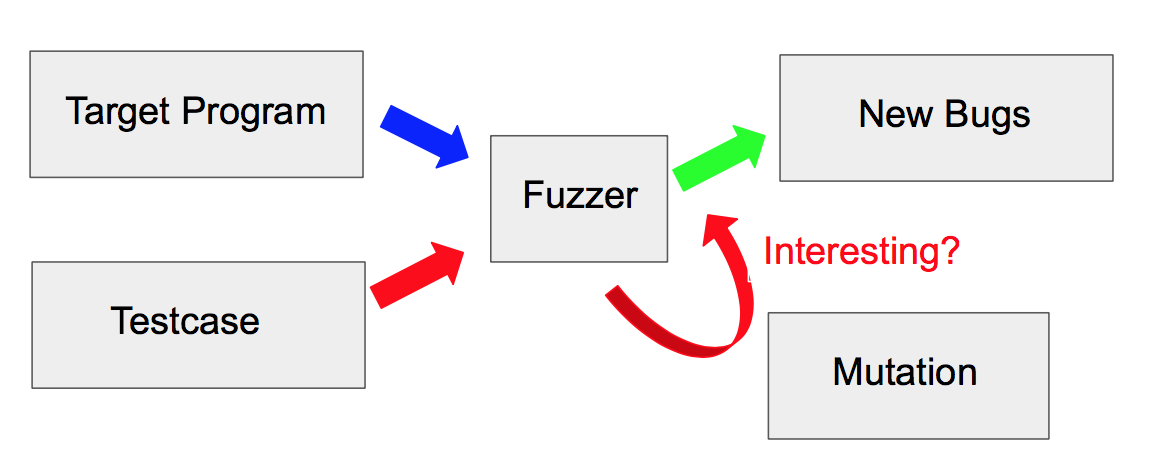
\includegraphics[scale=.4]{fuzzer_achitecture}
\caption{The basic architecture of a fuzzer.}
\end{figure}

During the loop of fuzzing, it collects a small corpus of interesting test cases, which are very important for seeding other new test cases. While fuzzing tools are generally aimed to explore and test undefined areas that may trigger bugs, how to get those test cases for an undefined area is the core problem. AFL uses coverage test as the standard to distinguish test cases. In another word, starts from that initial stage, it automatically discovers clean, interesting test cases by coverage test. AFL performs well to find some bugs, but it may take a relatively long time to trigger those interesting results. Some techniques, thus, are used to prevent redundant and repeated works by choosing different exploration paths as much as possible.


\section{Motivation}

While an important step of fuzzers, like AFL, is to repeatedly mutate the file using a balanced and well-researched variety of traditional fuzzing strategies, it is not trivial to recognize those clean and interesting test cases to do the real testing. If the test inputs generated by mutating cannot be effectively recognized as a repetition of an existing one, redundant work will be done again. 

The goal is to have an effective method to cover more program paths and trigger unexpected behavior. While the coverage test is used in the current version of AFL, we want to explore whether there's a better way as criteria. If we could reduce more repetition, the efficiency of AFL can be improved. In this project, we discuss a new approach to define whether a mutation of a test case is valuable and should be put into the queue for further mutation. We introduce invariants test instead of coverage test using a invariants detector, Daikon\cite{ernst2001dynamically}. 

The rest of paper is structured as follows. First, we discuss the related work. After that, we will illustrate the architecture of the invariant-based fuzzing method in details first. Then we will evaluate our approach using several testing programs and compare its performance with AFL. Some related work and future work are discussed after this. At last, a conclusion is given according to the previous discussion.

\section{Related Work}
\subsection{Fuzz testing}
Fuzz testing is an automated software testing technique. Depending on whether the fuzzers are aware of program structure, fuzzers could be categorized as white-, grey-, or black-box fuzzers.

Symbolic execution based white-box fuzzers like Klee\cite{cadar2008klee} or Katch\cite{marinescu2013katch} use symbolic program analysis and constraint solving to accurately direct the search in test generation as and when required.

American Fuzzy lop (AFL)\cite{gutmannfuzzing} is a coverage-based fuzzers. Unlike symbolic execution, AFL has the ability to generate lots of test cases. Its attempt to cover more program paths using mutations of seed inputs without incurring any overhead of program analysis. Some improvements have been introduced based on AFL. In the paper of AFL Fast\cite{ernst2001dynamically}, they present the structure of coverage-based Greybox Fuzzing (CGF). The recent work AFLGo\cite{bohme2017directed} is focusing on directed grey box fuzzing. It can achieve higher performance if there is a specific target to be tested. However, in our experiment, we apply the original edition of AFL because the possible application can be more general.

Since the AFL conduct random mutation to generate test cases, straying to the wrong direction can cause huge overhead. Combining the AFL to invariant-based testing can be a solution. Because the huge amount of test cases generated by mutation, the invariant-best testing tool can utilize those test cases to check whether they are in the range of current invariants. On one hand, those test cases remained can be applied on the invariant -best testing tool to produce more precise invariant; on the other hand, since the invariant-best testing tool delete some cases generated by AFL, the AFL can focus on those more promising routes.

\subsection{Discovering Program Invariants} 
Daikon\cite{ernst2001dynamically} can conduct dynamic inference of invariants for applications in software evolution. Dynamically inferred invariants also could be used in many situations that declared or statically inferred invariants can and, in some cases, the application of dynamic ones may be more effective. Invariants have many uses in computer science, and is considered as an indicator of triggering new running status of the program.Since the invariants generated by Daikon represent the current status of the program with input test cases, test cases which are out of the range of invariants are highly possible to discover a new path for the target program. It is thus a possible method to be used to eliminate useless data from the list of mutation test inputs from AFL. In addition, Daikon has the compatibility in C language which is ideal for integrating with AFL. Other tools that we considered such as Deduce\cite{hangal2002tracking}, are simpler than Daikon, but doesn't support C program.


\section{Technical approach}
In this project, we would like to apply the comparison of "invariants" in programs instead of just the criteria based on the coverage in AFL. The "invariants" here is not the true invariants for the program, but relatively unchanged variants compared with several inputs. To find the "invariants" in the program, we plan to use Daikon. Daikon is an implementation of dynamic detection of likely invariants, which are the properties hold by the given testing program at certain positions. For examples, x.field > abs(y), y = 2*x + 3, array a is sorted. During the detection process, the Daikon invariant detector reports likely program invariants. If the "invariants" detected by Daikon are different from the invariants from previous inputs, we save the mutation for future variations. We compare the total number of test cases mutated and the number of interesting test cases identified by coverage test from original AFL and by our invariants detection method.

Our implementation is based on the original AFL program and Daikon program. In AFL, the mutated test cases are pushed into a queue if they are considered "interesting". If a mutation triggers execution of a previously-uncovered path in the code under test, then that mutation is saved to the input pool for future variations. We want to replace the coverage test with the invariants test. We still use AFL program to generate random mutations based on the sample inputs in the current corpus. Instead of the coverage tests in original AFL, we use "invariants" to consider whether this test case should be use or not less by running Daikon and a comparison program implemented by ourselves. If certain test cases generates a new a set of "invariants" that differ from previous from Daikon, we consider it as the interesting test case. 

\begin{figure}[h]
\centering
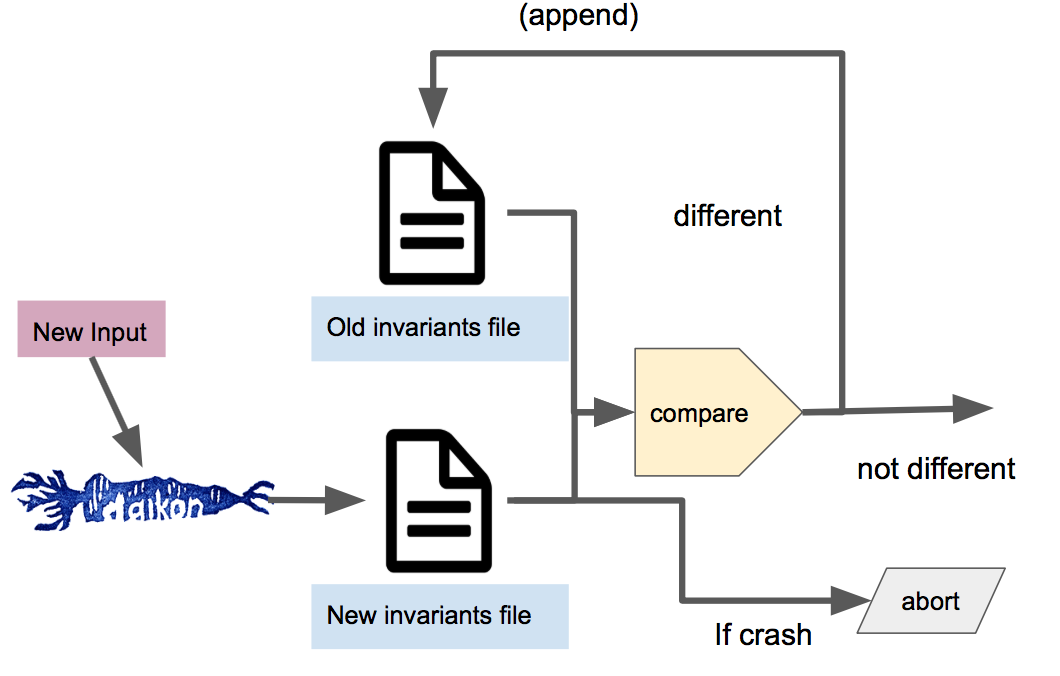
\includegraphics[scale=.45]{our_arc}
\caption{The architecture of the proposed fuzzer.}
\end{figure}

To determine whether it's a new interesting test case, we need to compare with all the test cases we have been seen. It's an expensive task in terms of running time and memory used. However, we found that in most of the cases, they only differ in a small number of invariants. In order to efficiently compare with all the previous test cases, the work around solution we proposed here is to see whether there exits new invariants that are not discovered. In another word, whether it's not contained in the file with all the previously detected invariants. We append all the unique invariants into a file we called "old invariants file". For the invariants detection process, there will be three possible outcomes:
\begin{enumerate}
\item found new invariants not contained in old invariants
\item all the invariants are contained in old invariants
\item a crash is reported
\end{enumerate}
For the first case, it's considered an interesting case, and we  append the new changes of "invariants" to the "old invariants file". Then we continue to test the program with new mutations. Not interesting test cases, or the second situation, will be ignored. If, however, this test case causes the target program to crash, which will be reported by Daikon, we abort the fuzz test and output the report. The report contains the information about how many test cases we have tested with and how many interesting test cases we have found.  

\section{Evaluation}
In this project, we would like to compare the original AFL with our modified AFL with invariants. The efficiency to find the bug is our evaluation criteria. The most common approach -- comparing by the computation time, however, is not an idea testing method to our case. Since we integrate two existing applications using native approach, the time consumption may largely due to the implementation instead of the algorithm. Other factors may also affect such as the hardware. Thus, the best criteria would be the testing iterations before targeting a new bug. In another word, we want to record how many test cases has been used in AFL to find the bug and compare this number.

In the implementation of AFL, the variable name "total paths" represent the test cases that have been executed. In the following evaluation, we conduct three experiments and compare the result of original AFL and the invariant--based AFL.

We design two simple example to that we think the invariant--based AFL might perform better than the original AFL. The first one is an integer overflow example. Since only the integer that is higher than the integer range will trigger this bug, if the original test case doesn't cause an integer overflow, the AFL will consider other test cases with a higher value as not interesting. The second example is a buffer overflow example. The bug will be triggered if the input length is longer than the input buffer. Since the AFL will also consider those inputs with different length as not interesting because the coverage is also the same, the invariant--based AFL might perform better in this example.

\subsection{Integer Overflow}

In computer programming, an integer overflow occurs when an arithmetic operation attempts to create a numeric value that is outside of the range that can be represented with a given number of bits. Integer overflow will make the value of integers that is larger than the maximum value become a negative value and vice versa. In C program, the maximum value of integer is $2^{31}-1 = 2147483647$ and the minimum value is $-(2^{31}) = -2147483648$.

In the experiment of integer overflow, we implement a simple binary search program which will trigger the integer overflow problem in some cases. The program can be seen in list 1.

\begin{lstlisting}[language=C, caption=Binary Search example]
int BS(int arr[],int l,int r,int x)
{
    while(l < r){
        int mid = (l*C+r*C)/(2*C);
        //C is a large constant.
        if(arr[mid] == x)
            return mid;
        if (arr[mid] > x) 
            r = mid - 1;
        else
            l = mid + 1;
   }
   return -1;
}
\end{lstlisting}

In this program, the addition of l and r might overflow if the summation of those two values is above the maximum of integer in C. In order to make this program easier to overflow, we multiply l and r with a large constant. Also, we reject all input other than integer as the input value of l and r.

In the experiment, we modified the constant of C from $2^{0}$ to $2^{30}$, to compare the efficiency of original AFL and the invariant--based AFL. The result is as figure 1. 

%Plot of overflow 
\begin{figure}[h]
\centering
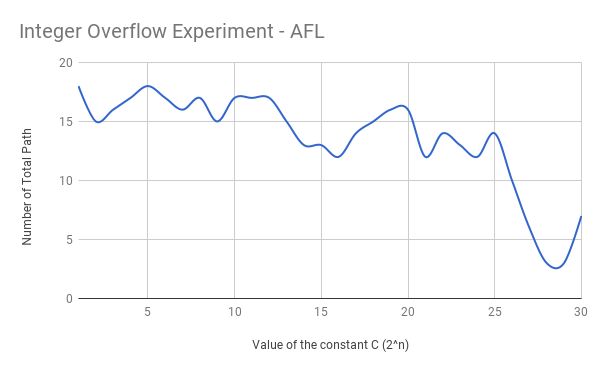
\includegraphics[scale=.4]{integer_AFL}
\caption{The x--axis represents the total paths that the AFL has been executed. The y--axis represents the value of the constant which is the power of 2. For example, if the point (5,17) represents the value of constant C is $2^{5}$ and the AFL executed 17 test cases to find the integer overflow bug.}
\end{figure}

According to the experiment result on integer overflow in AFL, it is really easy for AFL to find the bug in the binary search program. All of them find the bug within 20 test cases. Also, because AFL only tried few test cases, the bug was found in the first cycle. We can observe that if we increase the value of constant, AFL will find the bug within fewer cases. However, even though the constant is really small, it is still not very hard for AFL to find the integer overflow in this example.

\subsection{Buffer Overflow}

Buffer overflow attack gained notoriety in 1988 as part of the Morris Worm incident on the Internet \cite{spafford1989worm}. Despite the fact that
fixing individual buffer overflow vulnerabilities is fairly simple, buffer overflow attacks continue to this day \cite{cowan989stack}. In this experiment, we use a simple c program that will trigger the buffer overflow. The program is as Listing 2.

\begin{lstlisting}[language=C, caption=Buffer Overflow example]
int main(int argc, char *argv[])
{
    char name[5] = "";
    char lastname[10] ="";
    printf("Enter your name: ");
    scanf("%s", name);
    return 0;
}
\end{lstlisting}
In this program, the name array can only contain a limited amount of data, once the input string size is larger than the size of the name array, it will overflow to the last name part. In our implementation, we compare the last name array after the standard input, to check if it is the same as empty string. The program will return false if the last name array is corrupted.

In the experiment, we modified the length of name array. From 20 to 120, to compare the efficiency of original AFL and the invariant--based AFL. The result is as figure 2.

%Plot of buffer 
\begin{figure}[h]
\centering
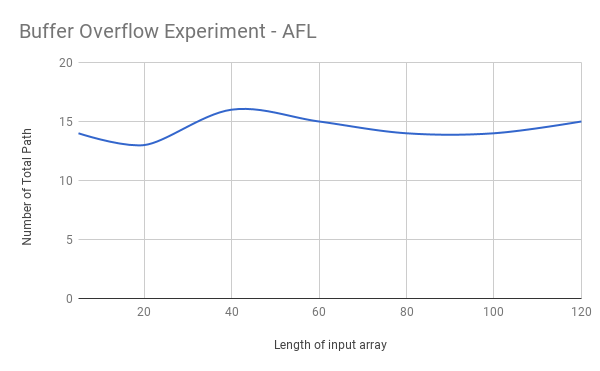
\includegraphics[scale=.4]{buffer_AFL}
\caption{The x--axis represents the test cases that the AFL have been executed. The y--axis represents the length of the input buffer. For example, if the point (5,14) represents the length of the input buffer is 5 and the AFL executed 14 test cases to find the buffer overflow bug.}
\end{figure}

According to the experiment result in the buffer overflow in AFL, it is also really easy for AFL to find the bug in this example. Out of our surprise, changing the length of the input buffer won't affect the running time of the AFL to find a bug really much. In figure 2, the buffer overflow bug can be detected within 16 test cases in all experimented length.

Base on the fact that AFL performs better than we expected, we added another test with memory corruption called FuzzGoat \cite{fgaddress} for AFL to test it's performance.

\subsection{Memory Corruption}
Fuzzgoat has been deliberately backdoored with several memory corruption bugs to test the efficacy of fuzzers and other analysis tools. The program was designed to load and process JSON data and then free the used memory. There are four potential vulnerabilities in the provided program. In order to compare the efficiency of the original AFL and the invariant--based AFL, we disassemble the original Fuzzgoat into four programs. Each program has a vulnerability inside. 
The four vulnerabilities are listed as follows:
\begin{enumerate}
\item Bug1: This line of code frees the memory referenced by *top, when the length is zero. If the program attempts to use that memory block later, it will cause an bug.
\begin{lstlisting}[language=C]
if (value->u.array.length == 0) 
    free(*top);

\end{lstlisting}
\item Bug2: This line of code incorrectly decrements the value of value->u.object.length. This may cause an invalid read when attempting to free the memory space.
\begin{lstlisting}[language=C]
if (!value->u.object.length) 
{   
    settings->mem_free (value->
    u.object.values, settings->
    user_data);
    break;
}
value = value->u.object.values [value
        ->u.object.length--].value;
\end{lstlisting}
\item Bug3: The code below decrements the pointer to the JSON string when the string is empty. The program then will try to call mem\_free on the pointer. It does not reference the JSON string.
\begin{lstlisting}[language=C]
if (!value->u.string.length)
    value->u.string.ptr--;
            
\end{lstlisting}
\item Bug4: The code below tries to dereference a NULL pointer when the length of string is equal to 1.
\begin{lstlisting}[language=C]
if (value->u.string.length == 1) 
{     
    char *null_pointer = NULL;
    printf ("%d", *null_pointer);
}
\end{lstlisting}
\end{enumerate}

We run the original AFL and the invariant--based AFL one by one to compare the efficiency.

%TODO put plot of fuzzgoat 
\begin{table}[h!]
\caption{Memory Corruption Experiment}
\begin{center}
\begin{tabular}{ |c|c| } 
\hline
Bug Name & Total Path \\
  \hline
  Bug1  & 99 \\ 
  Bug2 & 92 \\ 
  Bug3 & 57 \\
  Bug4 & 232 \\ 
  \hline
\end{tabular}
\end{center}
\end{table}

The total path in the table represent the test cases that have been executed by AFL when it found the first bug. Generally speaking, the original AFL can find all bugs in fewer than a hundred test cases. Notice that in bug 4, the AFL didn't find the bug. we executed it for 10 minutes and terminated it manually. It executed 232 test cases but didn't find the bug. It can be a possible future work to analyze the source code to further improve AFL.

\subsection{Invariant-based testing result}

\begin{table}[h!]
\caption{Invariant-based testing result}
\begin{center}
\begin{tabular}{ |c||c|c| } 
\hline
Test Program & Total Test Cases\\
  \hline
  Integer Overflow & $\approx 60$\\ 
  \hline
  Buffer Overflow & $\approx 60$\\ 
  
  \hline
\end{tabular}
\end{center}
\end{table}
Our implementation for invariant-base AFL fuzz, as described before, used AFL, Daikon and self-implemented algorithm to determine interesting cases. The part we used from AFL and Daikon can be executed successfully as instructed by the corresponding user manual. Our own implementation to compare the invariants has been proved to perform as we expected. To give more details, all the functions listed below are from the process, and they are all proved to meet the expectations. \begin{enumerate}
\item output the mutated test case from AFL(instead of doing coverage test) to be used for the next step
\item read the mutated test case and execute Daikon 
\item compare the invariants result based on this test case with the old invariants
\begin{enumerate}
\item Found crash
\item All invariants has been discovered before, then mark it as not interesting
\item Found new invariants, then mark it as interesting and add these new invariants to the set of old invariants.
\end{enumerate}
\item If the crash is found, abort the whole program and report the total number of mutated test cases and the number of interesting test cases.
\end{enumerate}
In order to prove that no duplicate test cases has been used, we keep track of all the test cases. The record showed us that all test cases are unique.\\
The results for invariant based AFL, however, are not fully tested for this experiment. The first problem is that it takes too long to run for one crash for one test program. This has been anticipated in the proposal because our naive implementation is not optimized. Our solution to this problem is to record and compare only how many test cases has been tried out, instead of execution time. However, the time consumed for one test was too long to allow us to finish the original testing plan. Only two test with "binary search" program and "enter name" program has been tested. The results for invariant based AFL are thus not displayed in the plotting as that of AFL.\\ 
The second problem is that the original AFL performs much better than invariant based AFL even in terms of the number of testing cycles. We didn't put all the test results for invariant based AFL here, because they are not better than the original AFL. We will mainly focus on the discussion about this result and thoughts for future works in the next section. \\


\section{Lessons learned and future work}
From our testing results, AFL performs well even with the test program that we intuitively not considered as suitable example to coverage test.
\begin{enumerate}
\item AFL uses other techniques other than coverage tests.
\item AFL implementation is optimized.
\item Fuzzing testing will mutate one test file many times and AFL uses optimized mutation methods. These example testing programs we use are still trivial and the bugs could be found within several mutation of one test file.
\end{enumerate}
There are some ways to optimize our implementation:
\begin{enumerate}
\item Implementation based on AFL code, which may not fit in well with the complicated and original code of AFL.
\begin{enumerate}
\item We directly use the mutation of test cases from AFL and ignore the coverage test results in AFL.
\item Maybe we ignored some other techniques, such as heuristic method, used by AFL.
\end{enumerate}
\item Maybe we are using the perfect way to detect and compare invariants.
\item Even though we tried with test cases that should favor invariants detection instead coverage test, it's possible there still exists sampling bias( which should be considered based on all the techniques used by AFL).
\end{enumerate}
There are future works that worth to be done before we make improvements on this project. 
\begin{enumerate}
\item Explicit research on how AFL works in terms of all the techniques implemented in their code, which includes:
\begin{enumerate}
\item How the mutation of test case works.
\item How exactly does AFL deal with interesting test cases.
\item What are the other techniques to try test cases with fuzz.
\end{enumerate}
\item How to use invariants test to identify interesting test cases.
\item By knowing what the expecting input test cases look like, it's possible to prune the test cases. With only valid input test cases, the total number of test cases that need to be tested can be largely reduced. This can reduce the time spent for running Daikon and comparison program.   
\end{enumerate}

\section{Conclusion}
In this paper, we present the structure that combines the AFL with invariants detection. We implemented a basic version to illustrate the idea and use some simple examples to prove it. Ideally, the invariant-based AFL can be utilized to detect several severer bugs like integer overflow, buffer overflow, and memory corruption. The future work can focus on the optimization of the invariant part. 


%% Bibliography
\bibliography{citations}


%% Appendix
%\appendix
%\section{Appendix}







\end{document}
